\subsection{Benchmark: Lorenz 1963}

We first verified that our choice of implementation for \glspl{esn}
produces similar results to those found in the literature \cite{pathak_using_2017}.
\begin{figure}[ht]
  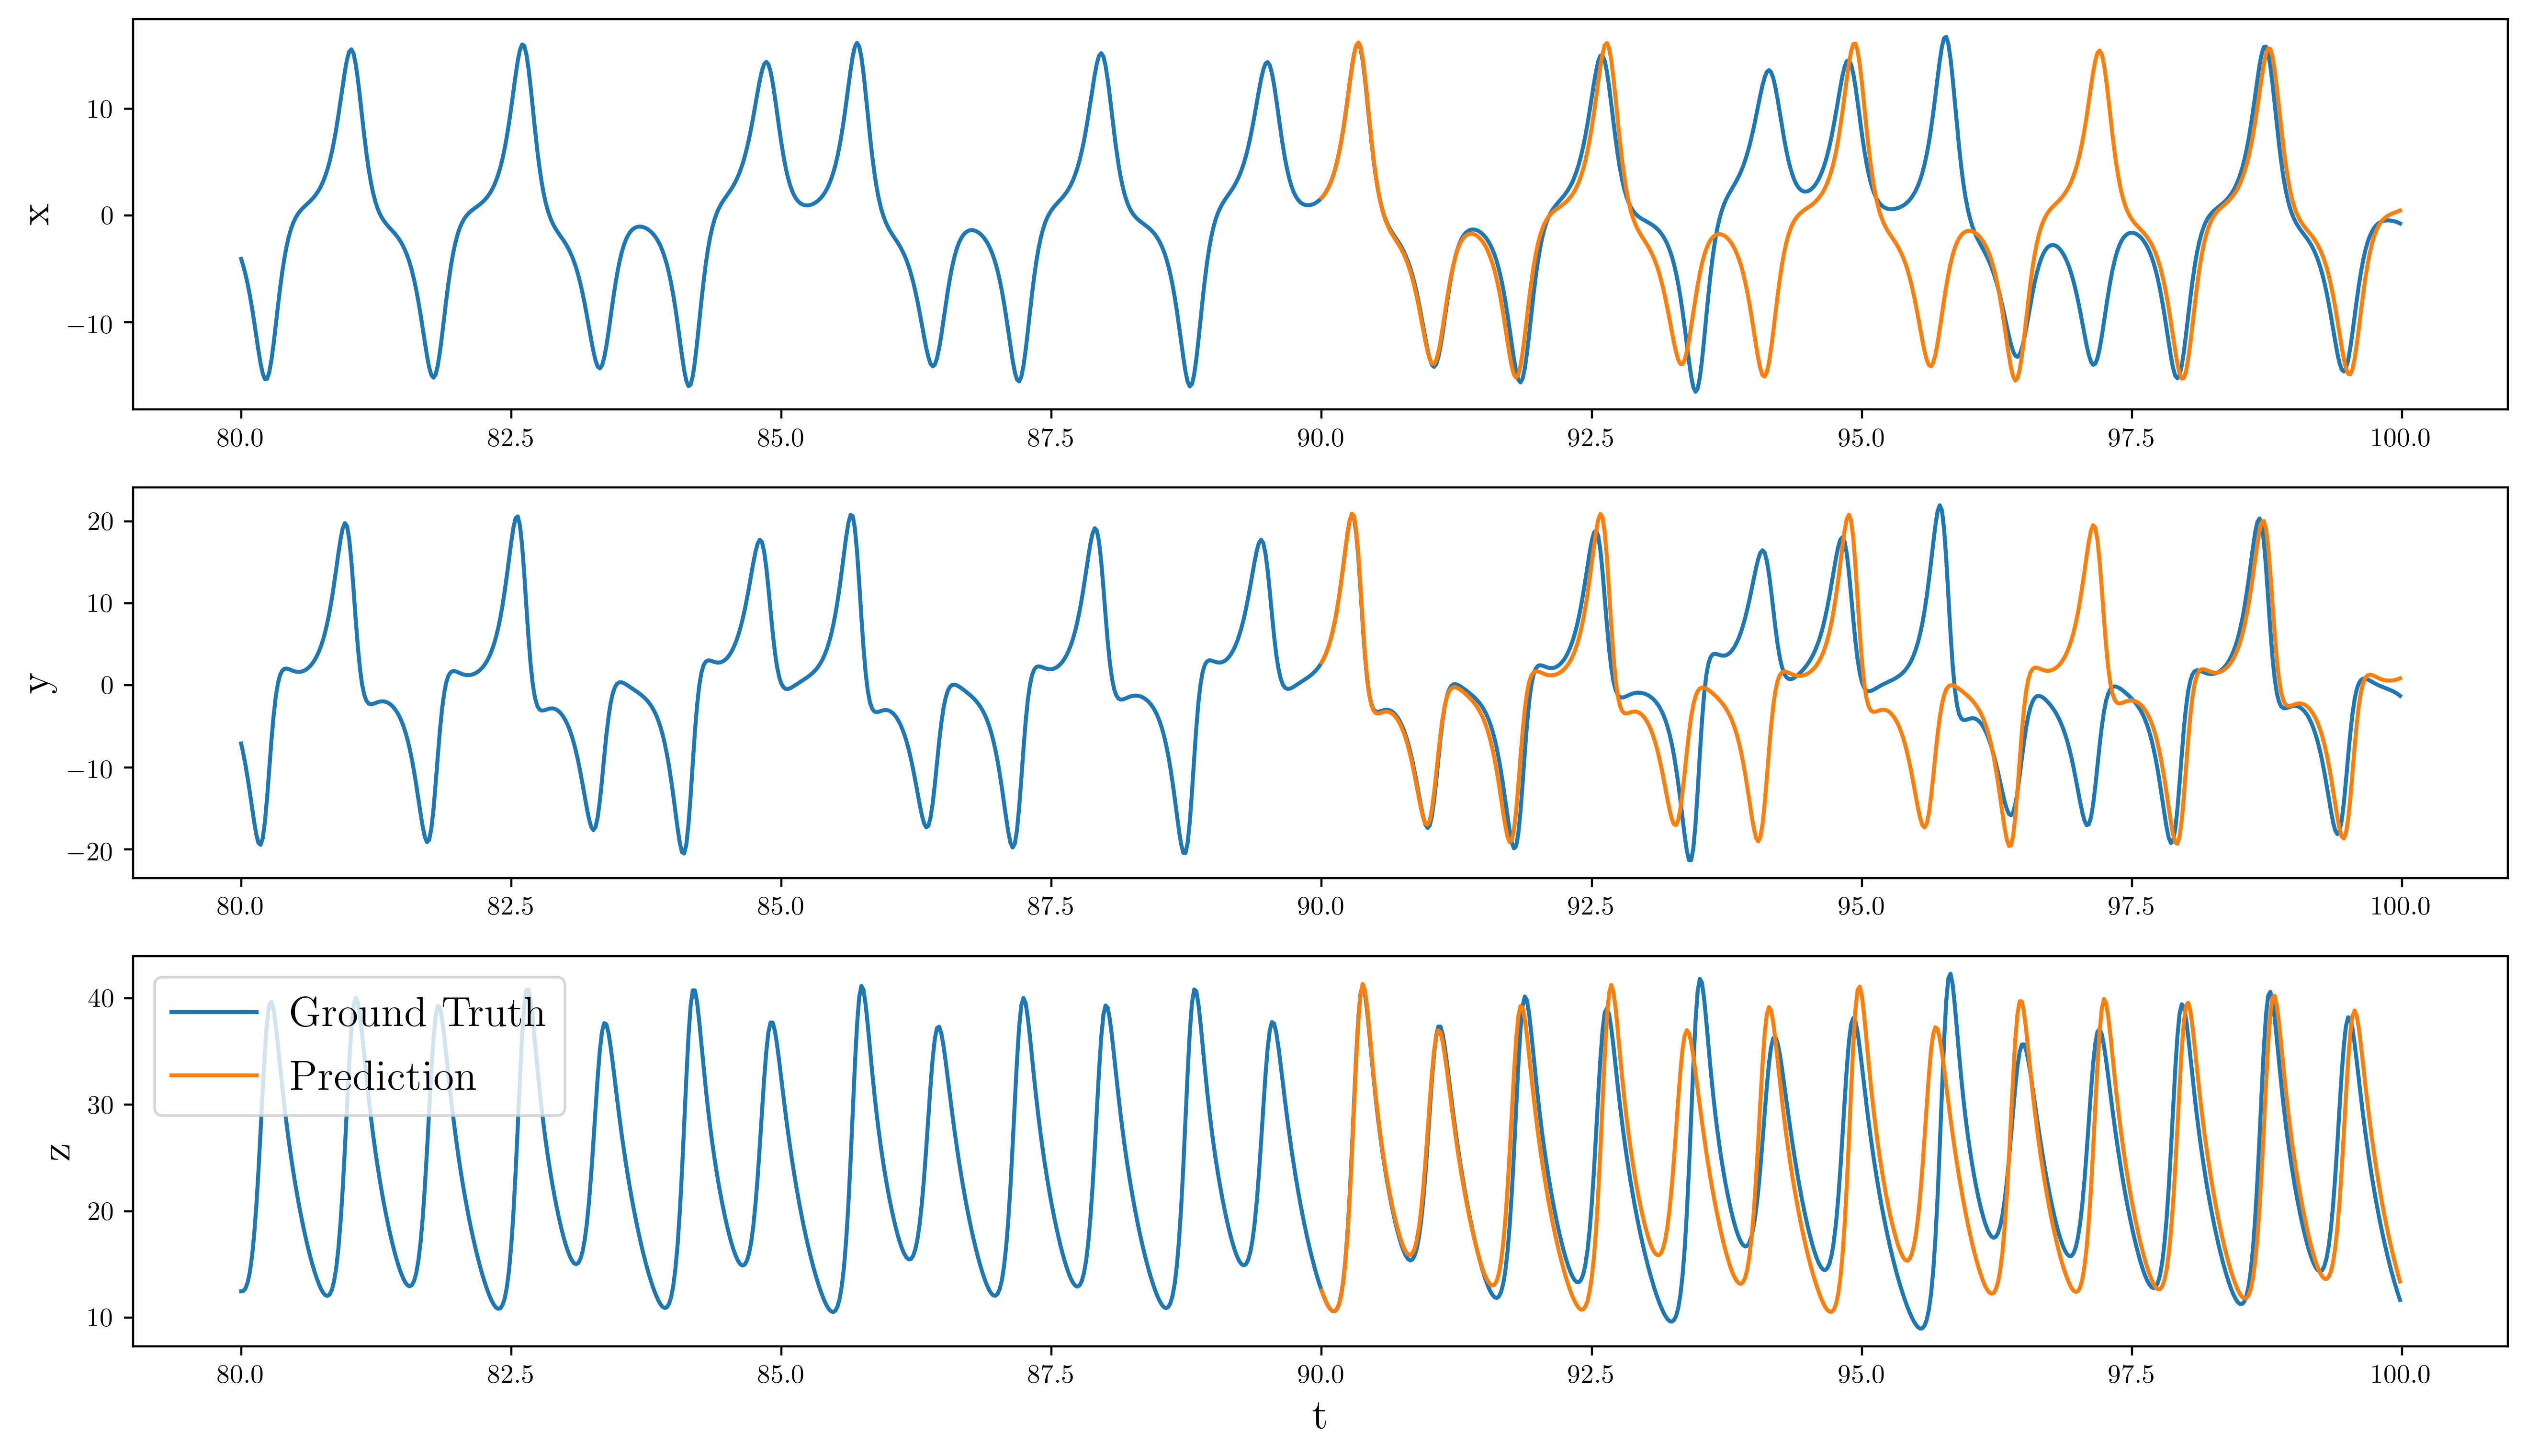
\includegraphics[width=\columnwidth]{lorenz63_prediction.png}
  \caption{Using an \gls{esn} to replicate the climate of the Lorenz Attractor.}
  \label{fig:lorenz63}
\end{figure}
The hyper-parameters that minimized the RMSE of the model can be found in Table
\ref{tab:lorenzparam}. Our optimized values are somewhat different from the literature, but we are satisfied that our \gls{esn} has succesfully
replicated the climate of the Lorenz Attractor similar to Pathak et. al 2017.
\begin{table}[ht]
  \centering
  \caption{Hyper-parameters for the Lorenz 1963 Model}
  \label{tab:lorenzparam}
  \begin{tabular}{c|c|c}
    \hline
    Parameter & This paper & Literature \cite{pathak_using_2017}\\
    \hline
    $N$ & 2000& 300\\
    $\rho$& 0.9&1.2\\
    \texttt{sparsity}& 0.1& 0.1\\
    \texttt{noise}& 0.001& 0\\
    Training Length & 3200& Not Specified\\
  \end{tabular}
\end{table}
